\chapter*{Introduzione}
\addcontentsline{toc}{chapter}{Introduzione}
Lo sviluppo sempre più rapido delle tecnologie di comunicazione ha imposto un nuovo modello di business che richiede sistemi sempre più affidabili che possano supportare ed agevolare tutte le attività di interscambio di dati ed informazioni. In particolare per alcuni sistemi critici, come quelli coinvolti nei pagamenti elettronici, è necessario adottare delle procedure per la protezione dei dati e dei sistemi al fine di garantire un livello di sicurezza adeguato alle criticità previste. Gli utilizzatori di questi servizi devono potersi fidare ed utilizzarli come intermediari tra le parti interessate.\newline\newline
Il concetto del \textit{tutto è connesso}\footnote{A partire dagli \textit{smart device} al mondo \textit{IoT} si ha un utilizzo massiccio di servizi cloud o web} apre nuovi scenari in cui la protezione e la gestione dei dati assume un ruolo fondamentale e spesso sottovalutato. Il caso di alcuni grandi \textit{data breach}\footnote{Un \textit{data breach} è una divulgazione, distruzione, perdita o modifica intenzionale od involontaria di informazioni sensibili protette al pubblico dominio; principalmente } e cattive gestioni dei dati personali\footnote{Il caso \href{https://www.nytimes.com/2017/09/07/business/equifax-cyberattack.html}{\textit{Equifax}} nel 2017 e lo scandalo di \href{https://www.washingtonpost.com/business/understanding-the-facebook-cambridge-analytica-story-quicktake/2018/04/09/0f18d91c-3c1c-11e8-955b-7d2e19b79966_story.html}{Facebook e Cambridge Analytica} nel 2018} ha portato ad una presa di consapevolezza su ciò che gli utenti scelgono di condividere con aziende, corporazioni, servizi ed altri utenti.\newline
Un esempio di questa diffusa consapevolezza è il crollo delle azioni di Facebook e l'abbandono del social-network a seguito della divulgazione dello scandalo di \textit{Cambridge Analytica} nel marzo del 2018: il motivo principale di questo discostamento è stata la perdita di fiducia in questa azienda che ha divulgato dati personali per di più di 50 milioni profili utente.\newline
\begin{figure}
    \centering
    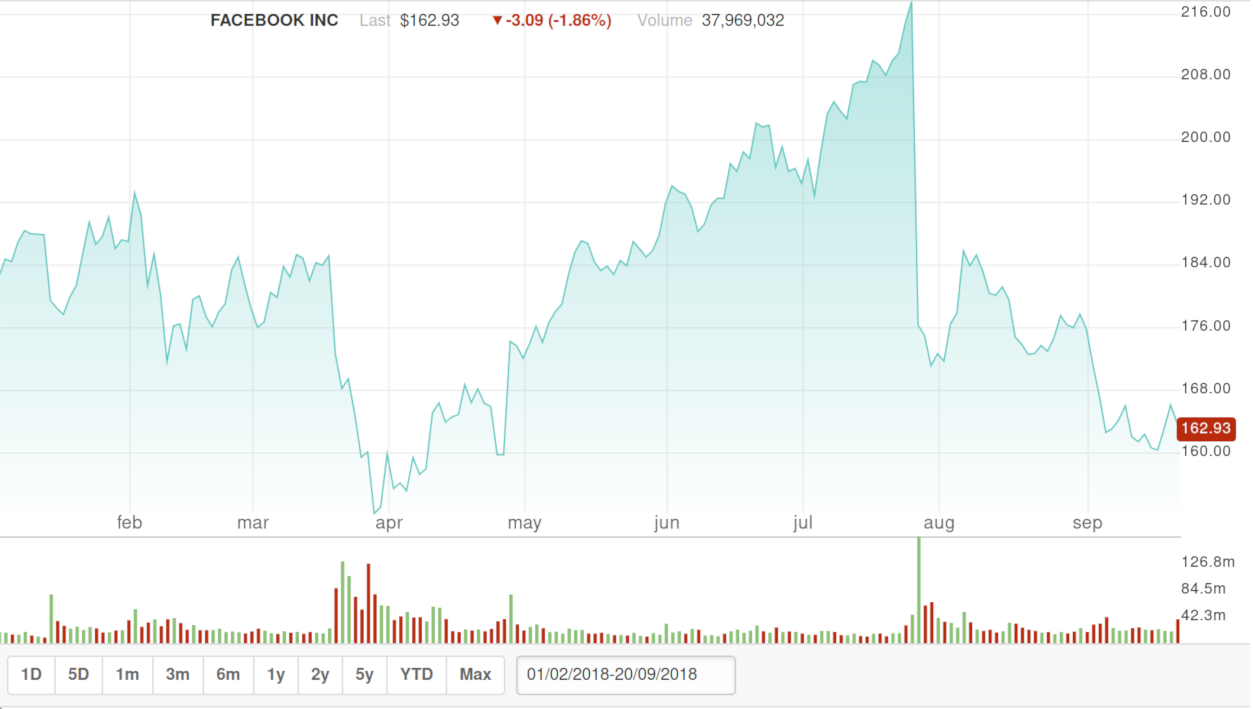
\includegraphics[width=\textwidth]{images/facebookstock.png}
    \caption{Grafico storico delle azioni di Facebook dal 1 Febbraio 2018 a 20 Settembre 2018}
    \source{Nasdaq}
\end{figure}
Una ulteriore conferma arriva dall'Unione Europea che ha stilato un regolamento sulla protezione dati: il \textit{GDPR}\footnote{\href{https://eur-lex.europa.eu/legal-content/IT/TXT/HTML/?uri=CELEX:32016R0679}{Regolamento (UE) 2016/679 del Parlamento Europeo e del Consiglio del 27 aprile 2016 relativo alla protezione delle persone fisiche con riguardo al trattamento dei dati personali, nonché alla libera circolazione di tali dati e che abroga la direttiva 95/46/CE (regolamento generale sulla protezione dei dati)}}; questo documento va ad aggiornare ed introdurre direttive e norme in fatto di privacy che erano rimaste invariate per venti anni risultando, quindi, obsolete.\newline

Queste tematiche di sicurezza, privacy, fiducia e sfruttamento dell'esperienza utente hanno messo in discussione le modalità in cui avvengono alcune interazioni online. I pagamenti online, ad esempio, avvengono tramite transazioni tra acquirente e venditore utilizzando dei servizi terzi come PayPal, Stripe, Google Wallet, Amazon Payments i quali conoscono i dettagli delle carte di credito degli utilizzatori e che usano per comunicare con i relativi istituti bancari funzionando da gateway tra venditore e acquirente.\newline
\begin{figure}
    \centering
    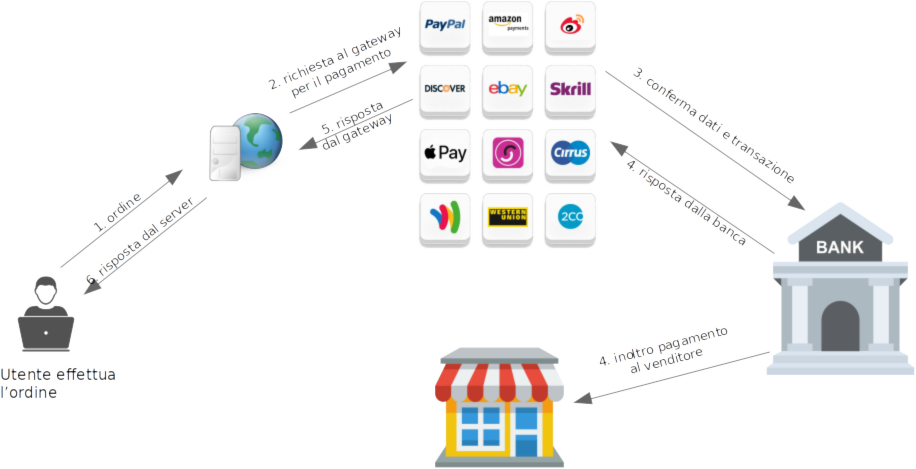
\includegraphics[width=\textwidth]{images/onlinepayments.png}
    \caption{Esempio di acquisto di beni con pagamenti gestiti da terzi}
\end{figure}
La comodità di questi servizi è indubbia ma viene persa la semplicità dell'interazione diretta con il venditore o il fornitore del servizio. In aggiunta è sempre opportuno considerare il rischio nella cessione di controllo sulle informazioni delle carte di credito o coordinate bancarie a servizi terzi e la perdita di privacy: ogni intermediario può costruire uno storico di transazioni per ogni utente.\newline\newline
Le preoccupazioni riguardo a privacy, sicurezza e decentralizzazione sono alcuni dei temi che hanno portato alla nascita di gruppi di attivisti chiamati \textit{Cypherpunk}\footnote{Il movimento \textit{Cipherpunk} nasce verso la fine degli anni '80 partendo da alcune idee proposte da \textit{David Chaum} su moneta digitale e sistemi di reputazione sena identità. Gli attivisti sostengono l'uso intensivo della crittografia e delle tecnologie atte a proteggere l'identità dell'utilizzatore per raggiungere un cambiamento sociale e politico che vada difendere la privacy delle persone anche ricorrendo alla forza ed agendo contro i governi.}. Essi sostengono l'uso intensivo della crittografia informatica come parte di un percorso sociale e politico al fine di riorganizzare i rapporti tra le persone e renderle più consapevoli nel proteggere il proprio diritto a privacy ed anonimato.\newline\newline
Uno degli obiettivi dell'attivismo \textit{Cypherpunk} è quello di creare dei sistemi di pagamento online che facciano ampio uso di meccanismi crittografici. Il principale motivo del distacco verso gli attuali metodi di pagamento è dovuto dalla mancanza di fiducia verso gli istituti bancari in quanto devono tener traccia privatamente, per ragioni di privacy e sicurezza, di ogni account e relativi spostamenti di denaro. Viene a crearsi quindi un sistema basato esclusivamente sulla fiducia: ogni partecipante deve fidarsi della banca per ogni transazione in quanto è l'istituto stesso che decide se rifiutarla od accettarla. In aggiunta dal punto di vista della sicurezza è possibile che agenti interni od esterni vadano ad alterare volontariamente dati sensibili con relativa perdita di denaro per la banca e i correntisti. Dal punto di vista dei \textit{Cypherpunk} l'unico modo per aver fiducia in un sistema è quello di \textit{obbligarlo} all'utilizzo di algoritmi crittografici sicuri.\newline\newline
A partire dagli anni '90, infatti, è cresciuto sempre più il numero di persone interessate a mantenere la propria identità riservata, anche per scopi malevoli\footnote{Spesso i servizi di anonimizzazione vengono fuorviati come servizi per nascondere la propria identità per scopi illegali o malevoli e non come possibili soluzioni a governi o regimi opprimenti che non garantiscono la libertà di parola.}, e che possono essere associate al movimento dei \textit{Cypherpunk}; nel caso dei pagamenti online sono stati molti i progetti proposti per avere un sistema di pagamento che metta in contatto direttamente venditore ed acquirente in maniera trasparente e senza intermediari, ovvero ``trustless'', garantendo al tempo stesso privacy e sicurezza. Molte proposte si sono rilevate incomplete\footnote{\textit{DigiCash} ad esempio permetteva agli acquirenti di restare anonimi ma ciò non era possibile per i venditori.} o inapplicabili\footnote{Negli Stati Uniti d'America era illegale, fino al 1992, esportare tecnologia crittografica per ragioni di sicurezza.} ma hanno costituito una forte base tecnologica e razionale a ciò che nel 2008 verrà proposto da \textit{Satoshi Nakamoto} nel \textit{whitepaper}: \textit{Bitcoin: A Peer-to-Peer Electronic Cash System}.\newline\newline
Il progetto proposto da Satoshi si impegna a risolvere il problema dei pagamenti online attraverso un sistema di consenso distribuito, decentralizzato e basato su incentivi attraverso dei meccanismi crittografici che vanno a costituire il nucleo fondamentale della valuta \textit{Bitcoin}: la \textit{blockchain}.\newline
Una \textit{blockchain} può essere vista come un database distribuito e replicato su diversi computer in rete capace di gestire transazioni monetarie in maniera del tutto decentralizzata.\newline\newline
La vera innovazione portata dalla tecnologia alla base dei \textit{Bitcoin} è la capacità di risolvere il \textit{problema dei Generali Bizantini}: raggiungere un consenso in situazioni in cui è possibile la presenza di errori.\newline
Il problema consiste nel trovare un accordo, comunicando solo tramite messaggi, tra componenti diversi nel caso in cui siano presenti informazioni discordanti\footnote{Il problema dei Generali Bizantini è esemplificato dalla situazione in cui tre o più generali debbano decidere se attaccare o ritirarsi dal campo di battaglia e decidendo all'unanimità. Esiste anche la possibilità che uno o più generali siano dei traditori e diffondano ordini discordanti. La soluzione al problema deve avvantaggiare i generali leali.}.\newline
\begin{figure}
    \centering
    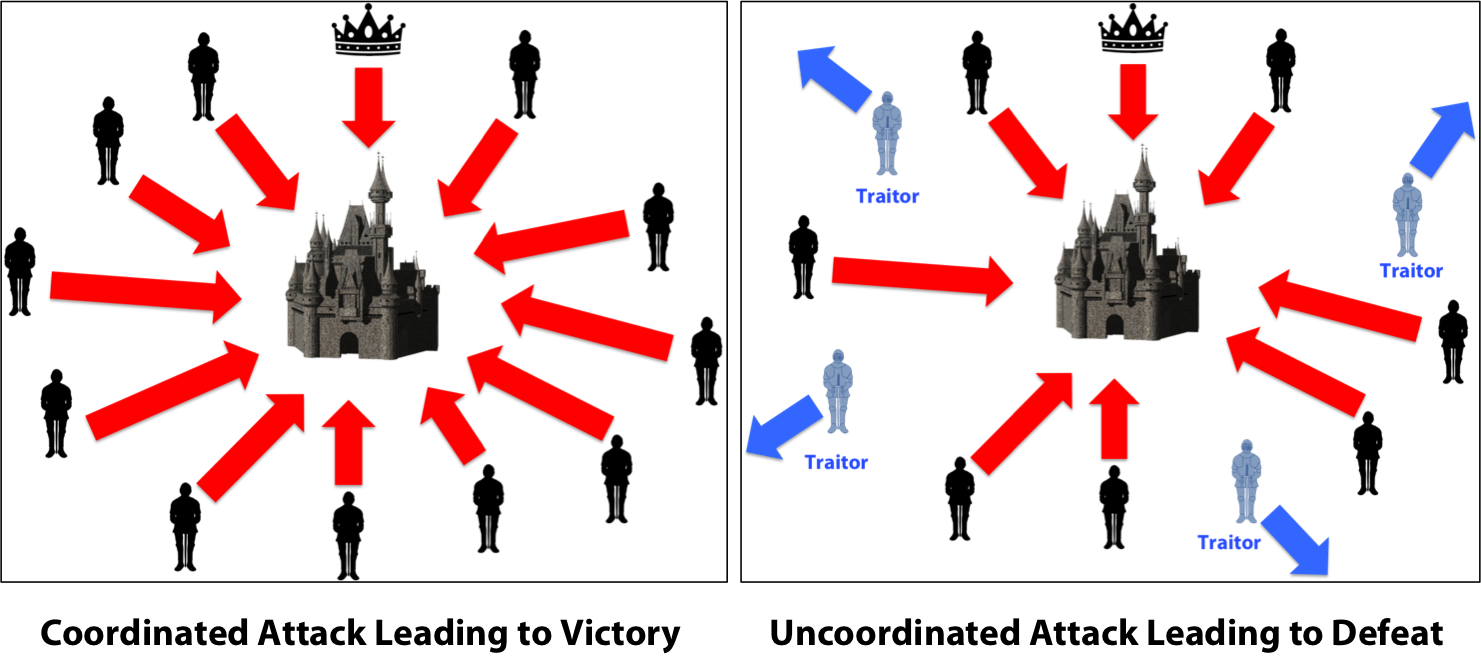
\includegraphics[width=0.8\textwidth]{images/byzantine.png}
    \caption{Schematizzazione di due scenari del problema dei Generali Bizantini}
    \source{\href{https://medium.com/@DebrajG/how-the-byzantine-general-sacked-the-castle-a-look-into-blockchain-370fe637502c}{Medium}}
\end{figure}
Oltre a garantire un sistema per lo scambio di valori ed informazioni il protocollo \textit{Bitcoin} permette che tutte le operazioni avvengano in maniera sicura evitando alcuni dei problemi riscontrati in precedenti progetti proposti tramite l'assunzione che se la maggioranza dei partecipanti delle rete ha buone intenzioni allora le entità malevoli hanno una possibilità di riuscita approssimativamente nulla.\newline
La validità assoluta di questa assunzione è dimostrabile solo in teoria in quanto non è ancora stato possibile verificarne l'effettiva correttezza sulla pratica a causa della complessità della rete e della componente randomica che viene utilizzata all'interno del protocollo: all'aumentare dei nodi diminuisce la possibilità di successo di un potenziale attacco e ne aumenta la complessità.\newline
È possibile, tuttavia, simulare alcuni scenari di attacco su blockchain e provare a definire delle soglie di rischio per cui la difficoltà delle riuscita di tale attacco risulti essere non trascurabile.\newline
L'obiettivo di questo progetto di tesi è quello di costituire un sistema che permetta agevolmente la possibilità di simulare le funzionalità basilari di una blockchain in un ambiente controllato che permetta di effettuare analisi di alcuni test di attacco fino ad ora basati solo su modelli teorici. Il modello deve evitare di restringere i vincoli imposti da un sistema controllato e non randomico in quanto è possibile ottenere dei falsi positivi, per esempio, usando un ridotto numero di peer può aumentare esponenzialmente le possibilità di successo di un attacco \textit{double-spending}\footnote{Quando un token può essere speso più di una sola volta a causa di una falla in uno schema per criptomonete; è il corrispettivo digitale della falsificazione di banconote.}.\newline
Il progetto e lo studio si focalizzano prevalentemente sulla blockchain per i Bitcoin in quanto la più diffusa ed utilizzata attualmente ma molti degli scenari proposti possono essere facilmente riadattati o configurati anche per altre criptomonete.
\begin{figure}[H]
    \centering
    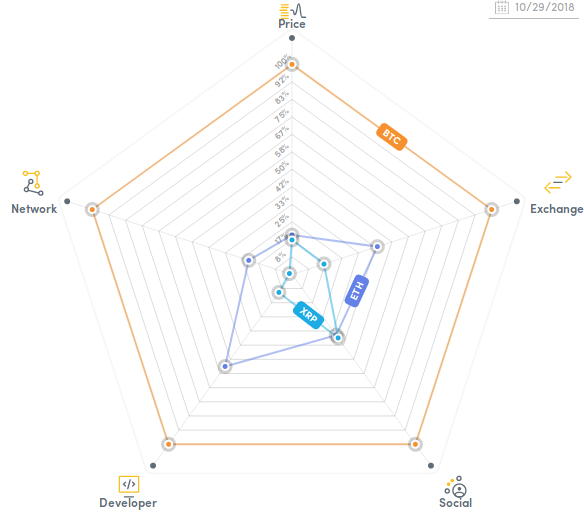
\includegraphics[width=0.85\textwidth]{images/crypto_economics.png}
    \caption{Confronto tra le tre principali criptomonete: \textit{Bitcoin}, \textit{Ethereum} e \textit{Ripple}. Il pentagono rappresenta il valore di mercato, il numero di transazioni, presenza nelle community e nei social, impegno degli sviluppatori e numero di nodi attivi.}
    \source{\url{coindesk.com}}
\end{figure}

% NeoTex: mainfile=main.tex:
